	%-----------------------
	\chapter{État de l'Art}
	\thispagestyle{empty}
	%-----------------------

		%-----------------------
		\section{Les solutions}
		%-----------------------

			%-----------------------
			\subsection{Solution 1}
			%-----------------------

A l’heure actuelle, Micro-ros n’est supporté que par 2 modèles de cartes Arduino, Arduino Portenta H7 M7 Core
\url{https://store.arduino.cc/portenta-h7} et Arduino Nano RP2040 Connect \url{https://docs.arduino.cc/hardware/nano-rp2040-connect}. 

Nous avons d'ailleurs vu qu'une personne a installé Micro ROS sur ces cartes : \url{https://www.youtube.com/watch?v=mq1uFGsYqeU}.

Il était probablement possible d’adapter Micro-ROS à la carte Arduino que nous avions à notre disposition mais cela risquait de nous 
prendre plus de temps que nous n’avions à disposition.  
\linebreak
	
L'Arduino Nano RP2040 Connect est une carte de développement basée sur le processeur ARM Cortex-M0+ RP2040 conçue par Raspberry Pi. 
Elle est conçue pour être petite, flexible et facile à utiliser pour les projets de robotique et d'Internet des objets (IoT). 
L'Arduino Nano RP2040 Connect est équipée de 20 broches de E/S numériques, de 6 broches PWM, de 6 broches analogiques, 
d'un port USB-C pour l'alimentation et la communication, d'un connecteur de batterie, d'un connecteur de microphone, 
d'un connecteur de haut-parleur et d'un connecteur de bouton-poussoir. La carte est également compatible avec les bibliothèques Arduino 
pour faciliter le développement de logiciels pour les projets de robotique et d'IoT. 
Après nos différentes recherches, nous avons conclu que ce serait la carte idéale pour mettre en place le projet.
\linebreak 

\begin{figure}[H]
\begin{center}
	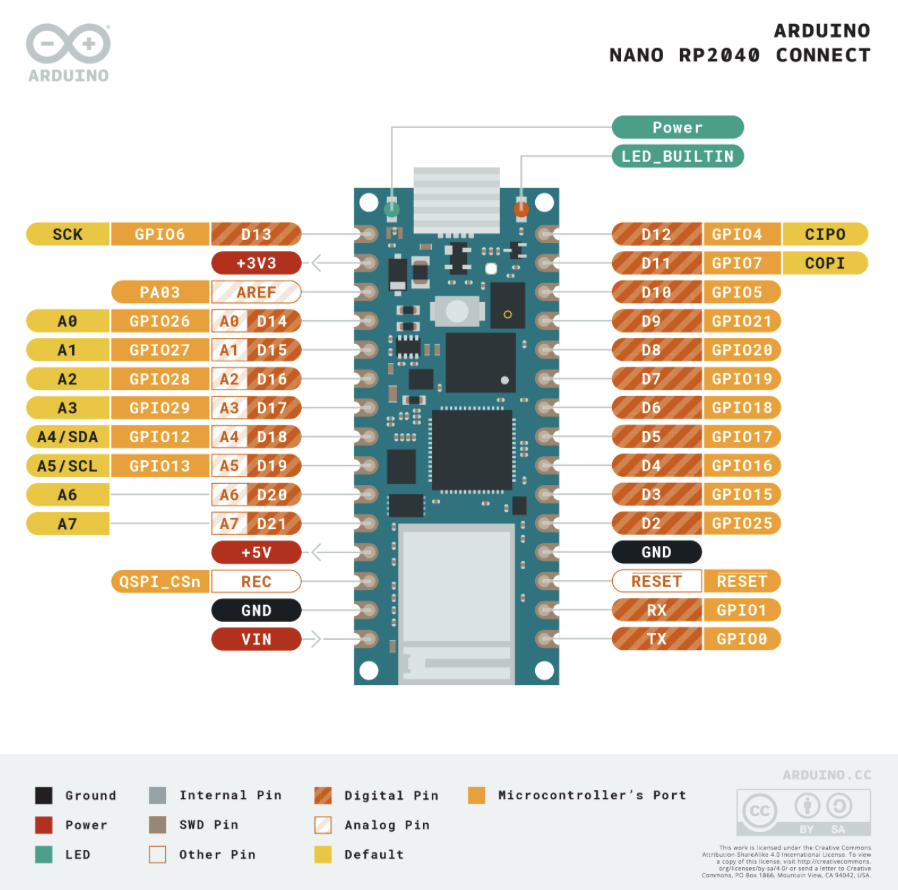
\includegraphics[width=0.7\textwidth]{./img/schema_carte_1}
\end{center}
\end{figure}

\begin{figure}[H]
\begin{center}
	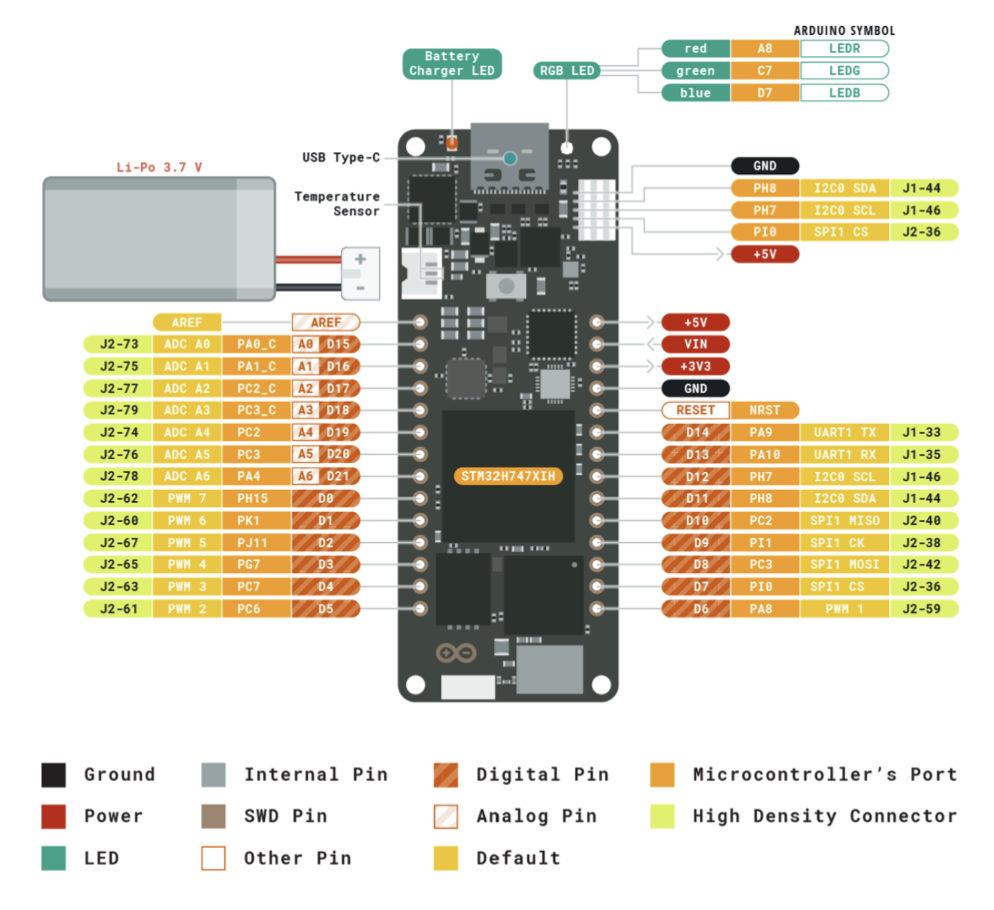
\includegraphics[width=0.7\textwidth]{./img/schema_carte_2}
\end{center}
\end{figure}

			%-----------------------
			\subsection{Solution 2}
			%-----------------------

Nous avons cependant pensé à une solution alternative. Nous pouvons aussi utiliser une carte ESP32 qui est déjà compatible 
avec l’architecture Micro-ROS ( \url{https://micro.ros.org/blog/2020/08/27/esp32} ).  
\linebreak

ESP32 est une puce de microcontrôleur à double cœur conçue par Espressif Systems. Elle est principalement utilisée 
dans les applications de robotique, d'Internet des objets (IoT) et de réseaux locaux sans fil (Wi-Fi et Bluetooth). 
La puce ESP32 est équipée d'un processeur principal Xtensa Dual-Core LX6, d'un processeur coprocesseur ultra-basse consommation, 
d'une mémoire SRAM de 520 Ko, d'une mémoire flash de 16 Mo, d'un module Wi-Fi 802.11b/g/n/e/i et d'un module Bluetooth v4.2. 
La puce ESP32 offre également de nombreux E/S numériques, analogiques et PWM, ainsi que des fonctionnalités avancées telles 
que le traitement du signal numérique, le traitement en temps réel, l'interface de caméra et l'interface de bus série. 
En raison de ses performances et de ses fonctionnalités avancées, la puce ESP32 est largement utilisée dans de nombreux projets de 
robotique et d'IoT.
\linebreak
	
On peut installer cette carte sur notre robot et la brancher directement en SPI (Serial Peripheral Interface) avec la carte Arduino Nano pour 
ne pas avoir à la connecter en radio ou en wifi.  
L’ESP32 s’occupera de faire tous les contrôles et enverra des ordres à la carte Arduino qui se contentera de les exécuter; 
Les problèmes que l’on pourrait rencontrer avec cette méthode sont le manque de place sur le robot, un poids peut-être trop important, ainsi 
qu’un manque d’alimention, l’alimentation actuelle du robot ne sera peut-être pas suffisante pour alimenter les deux cartes. 
\linebreak

		%-----------------------
		\section{Installation de ROS 2}
		%-----------------------

Nous allons détailler dans cette section comment installer ROS 2 sur Linux et Windows.
\linebreak

\underline{Sur Linux (Recommandé) :}
 
Suivre la documentation suivante :
\url{https://docs.ros.org/en/rolling/Installation/Ubuntu-Install-Debians.html}
 \linebreak

 \underline{Sur Windows :}
 
 \begin{enumerate}
	\item Téléchargez la dernière version de ROS2 depuis le site Web officiel de ROS (\url{https://index.ros.org/doc/ros2/}). 
	Sélectionnez la version de ROS2 qui convient à votre version de Windows (32 bits ou 64 bits). 

	\item Installez les outils de build Colcon en suivant les instructions du site Web de ROS 
	(\url{https://index.ros.org/doc/ros2/Installation/Colcon/}).
	Colcon est un outil de build utilisé pour compiler et intégrer les logiciels ROS2. 

	\item Créez un environnement de développement ROS2 en utilisant l'outil "ament" 
	(\url{https://index.ros.org/doc/ros2/Installation/Ament/}).
	Ament est un outil qui permet de gérer les dépendances et les environnements de développement pour les projets ROS2. 

	\item Installez les bibliothèques de support de Windows pour ROS2 en suivant les instructions du site Web de ROS 
	(\url{https://index.ros.org/doc/ros2/Installation/Windows-Support/}).
	Ces bibliothèques sont nécessaires pour exécuter ROS2 sur Windows. 

	\item Ajoutez les variables d'environnement ROS2 à votre système en suivant les instructions du site Web de ROS 
	(\url{https://index.ros.org/doc/ros2/Installation/Windows-Environment-Variables/}).
	Ces variables d'environnement sont nécessaires pour exécuter les commandes ROS2 et accéder aux outils et aux bibliothèques ROS2 
	depuis n'importe quel emplacement de votre système. 

	\item Vérifiez que ROS2 est correctement installé en exécutant la commande "ros2 run demo\_nodes\_cpp talker" depuis une 
	invite de commandes.
	Cette commande devrait exécuter un noeud "talker" de démonstration qui envoie des messages de test à un noeud "listener" de démonstration.
	Si la commande s'exécute correctement, cela signifie que ROS2 est correctement installé et configuré sur votre système.

	\item Vous pouvez maintenant commencer à développer vos propres applications ROS2 en suivant les tutoriels et les exemples disponibles 
	sur le site Web de ROS (\url{https://index.ros.org/doc/ros2/}).
	N'oubliez pas de configurer votre environnement de développement et de compiler vos logiciels avec Colcon avant de les exécuter.
\end{enumerate}

L'étape suivante est de générer l'agent Micro ROS et le lancer. On peut retrouver à cet effet un tutoriel à cette adresse :
\url{https://gist.github.com/Redstone-RM/0ca459c32ec5ead8700284ff56a136f7}
\linebreak

\clearemptydoublepage

